\frame{\frametitle{SUIT: Major Achievements}

\begin{itemize}
   \item{New Features in PDAC}
      \begin{itemize}
         \item{Search and display WISE single epoch sources}
         \item{Incorporated the DAX imgServ v1 in SUIT}
      \end{itemize}
   \item{Visualizaiton}
      \begin{itemize}
         \item{Search and display HiPS images}
         \item{Multiple scattered plots within one plotting area }
      \end{itemize}
   \item{Build and deployment}
      \begin{itemize}
         \item{Experimented with docker and Kubernetes}
         \item{Added Jenkins task to build Firefly docker image}
         \item{Added Jenkins tasks to deploy/destroy Firefly application as Kubernetes pod}
      \end{itemize}
   \item{Implemented embedded database HyperSQL for table data support in Firefly}
   \item{Updated 3rd party packages: React, Webpack ...}
   \item{Various improvements  and bug fixes}
\end{itemize}
}

\frame{\frametitle{SDSS HiPS images in Firefly}
\begin{center}
 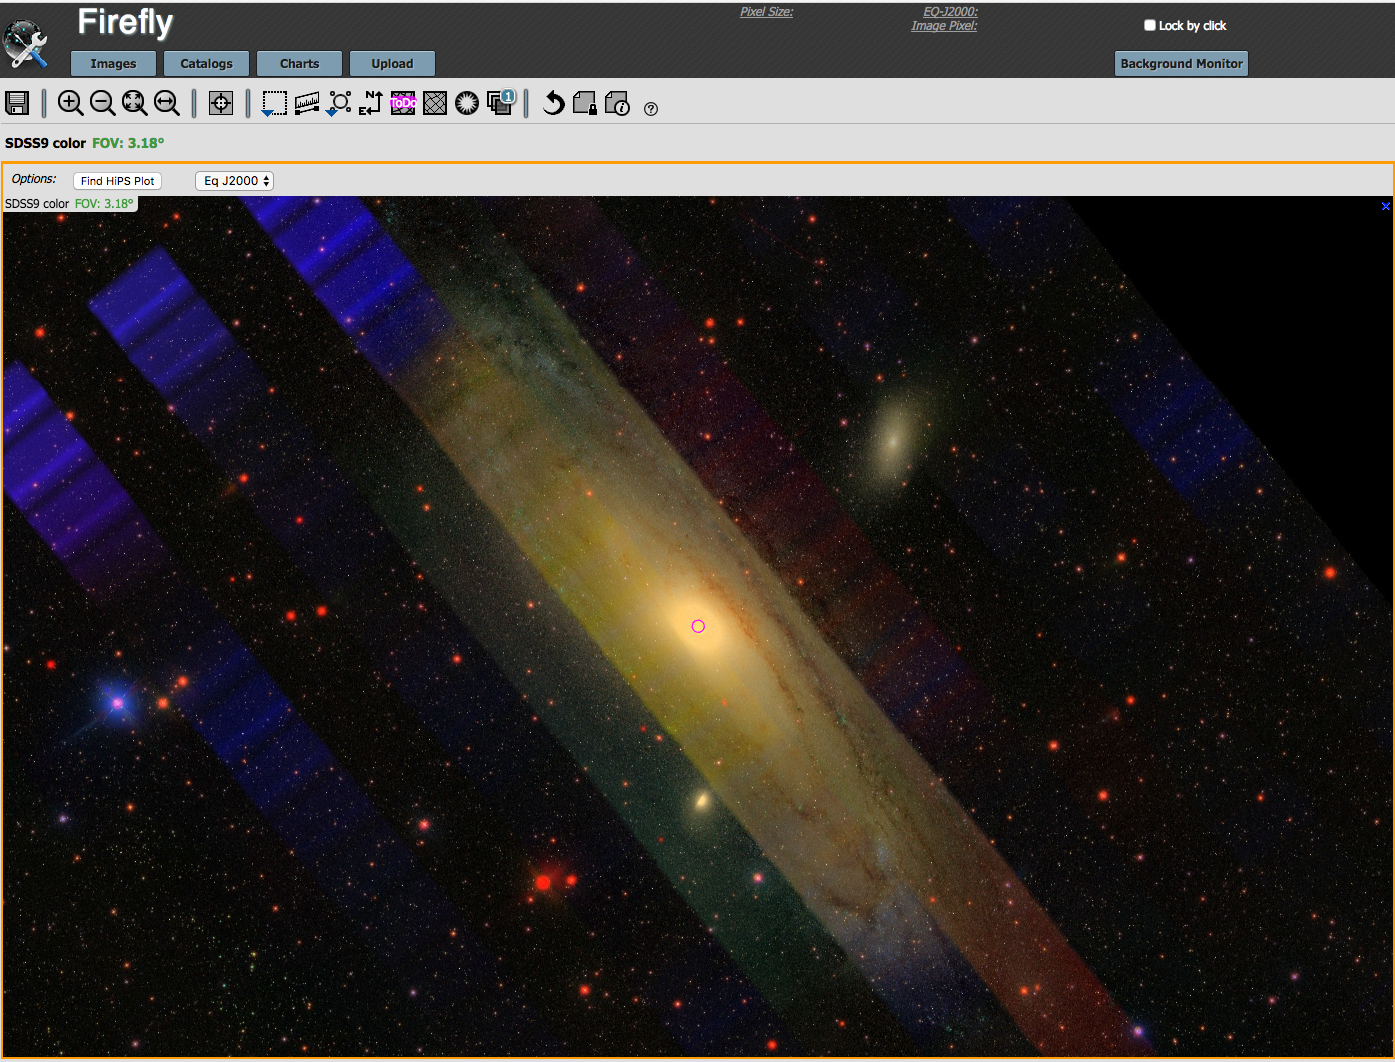
\includegraphics[width=0.7\textwidth]{sdssM31HEALPix1.png}
 \end{center}
}
\frame{\frametitle{SUIT: Plan for Next 6 Months}
\begin{itemize}
   \item{New Features in PDAC}
      \begin{itemize}
         \item {Search and display HSC data reprocessed by LSST pipeline}
         \item {Use the new version of DAX APIs: metaServ, imgServ, dbServ}
         \item {Integrate the authentication system}
         \item {Access workspace when available}
      \end{itemize}
   \item {Improve overall user experience in SUIT}
   \item {Make Firefly npm installable to support using Firefly API in JupyterLab}

\end{itemize}

}

